\documentclass[10pt,a4paper,twocolumn]{article}

% ==============================================================================
% Packages
% ==============================================================================
\usepackage[utf8]{inputenc}
\usepackage[T1]{fontenc}
\usepackage{newunicodechar}
\usepackage{libertinus}
\usepackage[margin=2cm]{geometry}
\usepackage{amsmath,amssymb,amsthm}
\usepackage{graphicx}
\usepackage{xcolor}
\usepackage[hyphens]{url}
\usepackage{hyperref}
\usepackage{booktabs}
\usepackage{tabularx}
\usepackage{multirow}
\usepackage{enumitem}
\usepackage{tikz}
\usepackage{pgfplots}
\usepackage{listings}
\usepackage{caption}
\usepackage{subcaption}
\usepackage{fancyhdr}
\usepackage{float}
\usepackage{placeins}  % For \FloatBarrier

% Float parameters to prevent overlapping
\setcounter{topnumber}{2}
\setcounter{bottomnumber}{2}
\setcounter{totalnumber}{4}
\renewcommand{\topfraction}{0.85}
\renewcommand{\bottomfraction}{0.85}
\renewcommand{\textfraction}{0.15}
\renewcommand{\floatpagefraction}{0.7}

% Prevent line breaks inside inline math (fixes broken superscripts/sqrt)
\relpenalty=10000
\binoppenalty=10000

\pgfplotsset{compat=1.18}
\usetikzlibrary{shapes,arrows,positioning,calc,patterns}

% ==============================================================================
% Colors and Styling
% ==============================================================================
\definecolor{codeblue}{RGB}{0,102,204}
\definecolor{codepurple}{RGB}{128,0,128}
\definecolor{codegreen}{RGB}{0,128,0}
\definecolor{codegray}{RGB}{128,128,128}
\definecolor{primaryblue}{RGB}{41,98,255}
\definecolor{warningred}{RGB}{220,53,69}
\definecolor{successgreen}{RGB}{40,167,69}

\hypersetup{
    colorlinks=true,
    linkcolor=primaryblue,
    citecolor=primaryblue,
    urlcolor=primaryblue
}

\lstset{
    basicstyle=\ttfamily\scriptsize,
    keywordstyle=\color{codeblue}\bfseries,
    commentstyle=\color{codegreen},
    stringstyle=\color{codepurple},
    numbers=left,
    numberstyle=\tiny\color{codegray},
    numbersep=4pt,
    xleftmargin=2em,
    framexleftmargin=2em,
    breaklines=true,
    frame=single,
    captionpos=b
}
\lstdefinelanguage{Solidity}{
    keywords={function, returns, return, if, else, for, while, do, break, continue, throw, require, revert, assert, public, private, internal, external, view, pure, payable, memory, storage, calldata, constant, immutable, virtual, override, modifier, event, emit, struct, enum, mapping, contract, interface, library, abstract, is, new, delete, true, false, uint256, uint128, uint64, uint32, uint16, uint8, uint240, uint224, int256, int128, int64, int32, int8, address, bool, bytes, bytes32, string, unchecked},
    sensitive=true,
    morecomment=[l]{//},
    morecomment=[s]{/*}{*/},
    morestring=[b]",
    morestring=[b]'
}

% ==============================================================================
% Theorem Environments
% ==============================================================================
\theoremstyle{definition}
\newtheorem{definition}{Definition}[section]
\newtheorem{property}{Property}[section]
\theoremstyle{plain}
\newtheorem{theorem}{Theorem}[section]
\newtheorem{lemma}[theorem]{Lemma}
\newtheorem{corollary}[theorem]{Corollary}
\theoremstyle{remark}
\newtheorem{remark}{Remark}[section]

% ==============================================================================
% Title and Authors
% ==============================================================================
\title{\textbf{\Large XPower Banq: Ring-Buffer Time Locks}\\[0.3em]
\normalsize A 16-Slot Quarterly Ring Buffer with $O(1)$ Depth Tracking\\
for Graduated Commitment in DeFi Lending}

\author{
    \textsc{Karun The Ritch}\thanks{\url{https://www.xpowerbanq.com}}
}

\date{}

\renewcommand{\thepage}{LCK/\arabic{page}}

% ==============================================================================
% Document Begin
% ==============================================================================
\begin{document}

\maketitle

% arXiv-style vertical tag on first page
\begin{tikzpicture}[remember picture, overlay]
  \node[rotate=90, anchor=center, font=\Huge, color=codegray]
    at ([xshift=1cm]current page.west)
    {preprint:2601~~[q-fin.CP]~~15 Mar 2026};
\end{tikzpicture}

% ==============================================================================
% Abstract
% ==============================================================================
\begin{abstract}
DeFi protocols benefit from knowing not just \emph{whether} tokens are locked but \emph{how long} they are committed. Naive implementations require $O(n)$ storage walks or unbounded gas. We present a 16-slot quarterly ring buffer that stores time-locked positions in constant per-slot storage with bitmap-guided $O(k)$ sweep ($k\leq 16$). The key contribution is an $O(1)$ cached depth metric: by storing the epoch-weighted sum $\Sigma = \sum v_i(e_i{+}1)$, exact token-seconds can be reconstructed via the algebraic identity $D = \Sigma \cdot Q - \mathit{timed}\cdot t + \mathit{perma}\cdot L$ using three \texttt{SLOAD}s and no iteration. Each lock requires 2--3 \texttt{SSTORE}s; each query requires 1--3 \texttt{SLOAD}s; proportional transfer runs in $O(k)$. The mechanism is deployed in the XPower Banq lending protocol~\cite{wp}, where the token-second depth drives graduated lock bonus/malus on interest rates.
\end{abstract}

\textbf{Keywords:} time-locked positions, ring buffer, token-seconds, DeFi lending, graduated commitment, Solidity

% ==============================================================================
% 1. Introduction
% ==============================================================================
\section{Introduction}
\label{sec:introduction}

Time-locked positions are a recurring primitive in DeFi. Vote-escrow protocols (Curve veCRV~\cite{curve}), liquid staking wrappers (Convex vlCVX~\cite{convex}), and lending protocols all require users to commit tokens for a bounded duration. Beyond binary locked/unlocked status, protocols benefit from a measure of \emph{commitment depth}---the integral of locked amount over remaining time, which we call \emph{token-seconds}.

Computing token-seconds on-chain presents a tension: the naive $O(n)$ summation over all lock entries is unbounded in gas, while maintaining a single aggregated counter sacrifices the ability to support multiple concurrent locks with different expiry dates.

\textbf{Contributions.} We resolve this tension with two mechanisms layered on a shared ring-buffer data structure:

\begin{enumerate}[leftmargin=*]
\item \textbf{Ring-Lock}: A 16-slot quarterly ring buffer with a bitmap-guided $O(k)$ sweep for expired slots, providing bounded-gas lock creation and expiry (Section~\ref{sec:ringlock}).

\item \textbf{Time-Lock}: An extension that adds a single stored value---the epoch-weighted sum $\Sigma = \sum v_i(e_i{+}1)$---enabling $O(1)$ reconstruction of exact token-seconds via an algebraic identity (Section~\ref{sec:timelock}).
\end{enumerate}

The protocol context is the XPower Banq lending protocol~\cite{wp}, where lock depth drives graduated interest rate adjustments (Section~\ref{sec:integration}). The locked-positions mechanism is described in~\cite{wp}~\S4.1 and the interest rate application in~\cite{wp}~\S4.7. Formal proofs of the ring-buffer invariants and depth identity appear in Section~\ref{sec:proofs}. A companion document~\cite{apx} provides extended mathematical analysis.

% ==============================================================================
% 2. Related Work
% ==============================================================================
\section{Related Work}
\label{sec:related}

\textbf{Curve veCRV}~\cite{curve}. Fixed 4-year linear decay from a single lock slot. $O(1)$ query via closed-form decay, but no support for multiple concurrent locks or variable duration. The bias/slope model requires periodic global checkpoints.

\textbf{Convex/Aura vlCVX}~\cite{convex}. Epoch-based unlock queues with linear scan for expired epochs. Supports multiple lock durations, but sweep cost is $O(n)$ in the number of distinct epochs---unbounded without a cap on lock granularity.

\textbf{Uniswap v3 NFT Locks.} Per-position NFTs carry individual timestamps. No aggregation across positions; each lock is an independent storage entity.

\textbf{OpenZeppelin TimelockController}~\cite{oz-timelock}. Designed for governance action delays, not position locks. Single-use: one pending action per hash, no ring or aggregation structure.

\textbf{Ring Buffers.} Circular buffers are classical in systems programming~\cite{ring-buffer}: OS scheduling, network packet buffers, Uniswap~V3 oracle observation arrays. Our application to on-chain time locks with bitmap-guided sweep and cached depth appears to be novel.

\begin{table}[htbp]
\centering
\caption{Comparison of time-lock mechanisms.}
\label{tab:comparison}
\small
\begin{tabular*}{0.95\columnwidth}{@{\extracolsep{\fill}}lccccc@{}}
\toprule
& Duration & Storage & Lock & Query & Depth \\
& Range & per User & Cost & Cost & Metric \\
\midrule
veCRV & Fixed 4y & 1 word & $O(1)$ & $O(1)$ & Linear \\
vlCVX & Epochs & $O(n)$ & $O(1)$ & $O(n)$ & None \\
NFT & Any & $O(n)$ & $O(1)$ & $O(n)$ & None \\
\textbf{Ours} & $[0,16Q)$ & 19 words & $O(1)$ & $O(1)$ & Token$\cdot$s \\
\bottomrule
\end{tabular*}
\end{table}

% ==============================================================================
% 3. Preliminaries
% ==============================================================================
\section{Preliminaries}
\label{sec:preliminaries}

\subsection{Definitions}
\label{subsec:definitions}

\begin{definition}[Epoch]
\label{def:epoch}
The \emph{absolute epoch index} at timestamp~$t$ is $e = \lfloor t / Q \rfloor$, where $Q = \texttt{LOCK\_TERM} \approx 91.3$~days (one calendar quarter).
\end{definition}

\begin{definition}[Slot Index]
\label{def:slot-index}
The ring-buffer \emph{slot index} for epoch~$e$ is $i = e \bmod 16$.
\end{definition}

\begin{definition}[Lock Expiry]
\label{def:lock-expiry}
A lock in epoch~$e$ expires at timestamp $(e{+}1) \times Q$, the start of the next epoch.
\end{definition}

\begin{definition}[Token-Seconds]
\label{def:token-seconds}
The \emph{token-second depth} for user~$u$ at timestamp~$t$ is:
\begin{equation}
\label{eq:token-seconds}
D(u,t) = \sum_{i \in A} v_i \bigl((e_i{+}1)Q - t\bigr) + p \cdot L
\end{equation}
where $A$ is the set of active (non-expired) timed slots, $v_i$ and $e_i$ are the value and epoch of slot~$i$, $p = \texttt{perma}[u]$ is the permanently locked amount, and $L = \texttt{LOCK\_TIME} = 16Q \approx 48$~months.
\end{definition}

\subsection{Storage Layout}
\label{subsec:storage-layout}

The complete storage is 19 words per user:

\begin{lstlisting}[language=Solidity, caption={Lock storage layout}, label={lst:lock-struct}]
struct LockSlot {
    uint32 epoch;  // absolute epoch index
    uint224 value; // locked amount
}  // 1 word (256 bits packed)

struct Lock {
    // 16-slot quarterly ring buffer
    mapping(address => LockSlot[16]) slots;
    // permanent (irrevocable) locked amount
    mapping(address => uint256) perma;
    // [uint240 total | uint16 bits]
    mapping(address => uint256) coded;
    // epoch-weighted sum: sigma v_i*(e_i+1)
    mapping(address => uint256) depth;
}
\end{lstlisting}

The first 18 words (16~slots + \texttt{perma} + \texttt{coded}) constitute the Ring-Lock layer. The \texttt{depth} mapping is the Time-Lock extension.

\subsection{Bitmap Encoding}
\label{subsec:bitmap}

The \texttt{coded} word packs two values: the upper 240 bits store the cached total locked amount, and the lower 16 bits store the active-slot bitmap. Decoding:
\begin{align}
\texttt{total} &= \texttt{coded} \gg 16 \label{eq:decode-total} \\
\texttt{bits} &= \texttt{coded} \mathbin{\&} \texttt{0xFFFF} \label{eq:decode-bits}
\end{align}

LSB extraction uses a de Bruijn sequence~\cite{debruijn}: the lowest set bit is isolated via $\texttt{lsb} = b \mathbin{\&} (\lnot b + 1)$, then multiplied by the constant \texttt{0x09AF} modulo $2^{16}$, producing a unique 4-bit hash in the top nibble that indexes into a 64-bit lookup table. This replaces 16 conditional \texttt{SLOAD}s with 1~\texttt{SLOAD} plus bit arithmetic.

% ==============================================================================
% 4. Ring-Lock Mechanism (RING_LOCK)
% ==============================================================================
\section{Ring-Lock Mechanism}
\label{sec:ringlock}

This section describes the base ring-buffer operations without depth tracking. Each subsection presents the algorithm, a TikZ figure of the ring-buffer state change, and a complexity analysis.

% ---------- 4.1 more() ----------
\subsection{\texttt{more(user, amount, dt\_term)} --- $O(1)$ Lock Addition}
\label{subsec:more}

\begin{figure}[htbp]
\centering
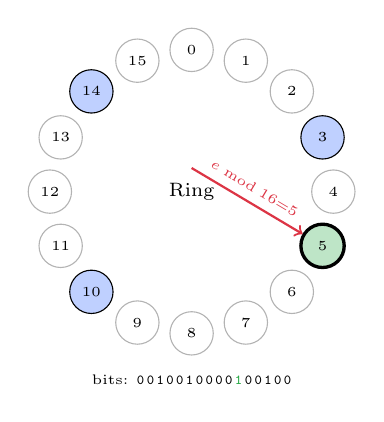
\begin{tikzpicture}[
    slot/.style={draw, minimum size=0.55cm, circle, font=\tiny, inner sep=0pt},
    active/.style={slot, fill=primaryblue!30},
    target/.style={slot, fill=successgreen!30, very thick},
    empty/.style={slot, draw=codegray!60},
]
    % Ring of 16 slots — empty
    \foreach \i in {0,1,2,4,6,7,8,9,11,12,13,15} {
        \pgfmathsetmacro{\angle}{90 - \i * 22.5}
        \node[empty] (s\i) at (\angle:1.8cm) {\i};
    }
    % Active slots
    \foreach \i in {3,10,14} {
        \pgfmathsetmacro{\angle}{90 - \i * 22.5}
        \node[active] (s\i) at (\angle:1.8cm) {\i};
    }
    % Target slot
    \pgfmathsetmacro{\angle}{90 - 5 * 22.5}
    \node[target] (s5) at (\angle:1.8cm) {5};
    \node[font=\scriptsize] at (0,0) {Ring};
    % Arrow to target
    \draw[->, thick, warningred] (0,0.3) -- (s5) node[midway, above, font=\tiny, sloped] {$e \bmod 16{=}5$};
    % Bitmap below
    \node[font=\tiny, anchor=north] at (0,-2.2) {bits: \texttt{0\,0\,1\,0\,0\,1\,0\,0\,0\,0\,\textcolor{successgreen}{1}\,0\,0\,1\,0\,0}};
\end{tikzpicture}
\caption{\texttt{more()} --- the target epoch maps to slot~5; existing active slots (3,\,10,\,14) are unaffected.}
\label{fig:more}
\end{figure}

The idea is straightforward: given a lock duration, compute which future epoch the tokens will expire in, then map that epoch to one of the 16~ring-buffer slots via modular arithmetic.  If the slot already holds tokens for the same epoch, the new amount is simply added; if it is stale (left over from a previous cycle), the old residue is cleaned up first---this ``self-healing'' step keeps the cached total consistent without requiring a separate garbage-collection pass.

\textbf{Algorithm.}
\begin{enumerate}[leftmargin=*, nosep, start=0]
\item Require $\texttt{amount} \leq 2^{224}{-}1$ and $\texttt{dt\_term} > 0$. Revert otherwise.
\item If $\texttt{dt\_term} = 2^{256}{-}1$ (sentinel): execute \textbf{permanent path}---add to \texttt{perma} and \texttt{coded} total; no slot write, no bitmap change. Return. \emph{(Early exit avoids overflow in the addition $t + \texttt{dt\_term}$ below.)}
\item Require $\texttt{dt\_term} \leq L - Q$. Revert otherwise.
\item Compute target epoch: $e = \lfloor(t + \texttt{dt\_term}) / Q\rfloor$.
\item Compute slot index: $i = e \bmod 16$.
\item If \texttt{slot.epoch} $\neq e$ (stale or empty):
    \begin{itemize}[nosep]
    \item If the old value is positive, subtract it from \texttt{total} (self-healing).
    \item Overwrite: \texttt{slot.epoch} $\leftarrow e$, \texttt{slot.value} $\leftarrow$ \texttt{amount}.
    \end{itemize}
\item If \texttt{slot.epoch} $= e$ (accumulate): \texttt{slot.value} $\mathrel{+}=$ \texttt{amount}.
\item Update \texttt{coded}: add \texttt{amount} to total, set bit~$i$.
\end{enumerate}

\textbf{Complexity}: 2~\texttt{SSTORE}s (slot~+ coded). Permanent: 2~\texttt{SSTORE}s (perma~+ coded).

% ---------- 4.2 free() ----------
\subsection{\texttt{free(user)} --- $O(k)$ Expired Slot Sweep}
\label{subsec:free}

\begin{figure}[htbp]
\centering
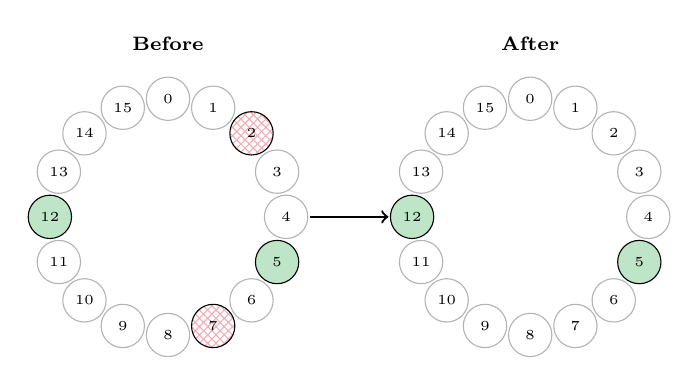
\begin{tikzpicture}[
    slot/.style={draw, minimum size=0.55cm, circle, font=\tiny, inner sep=0pt},
    active/.style={slot, fill=successgreen!30},
    expired/.style={slot, fill=warningred!20, pattern=crosshatch, pattern color=warningred!40},
    empty/.style={slot, draw=codegray!60},
]
    % Before ring
    \begin{scope}[xshift=-2.3cm]
    \node[font=\scriptsize] at (0,2.2) {\textbf{Before}};
    \foreach \i in {0,1,3,4,6,8,9,10,11,13,14,15} {
        \pgfmathsetmacro{\angle}{90 - \i * 22.5}
        \node[empty] (b\i) at (\angle:1.5cm) {\i};
    }
    \foreach \i in {2,7} {
        \pgfmathsetmacro{\angle}{90 - \i * 22.5}
        \node[expired] (b\i) at (\angle:1.5cm) {\i};
    }
    \foreach \i in {5,12} {
        \pgfmathsetmacro{\angle}{90 - \i * 22.5}
        \node[active] (b\i) at (\angle:1.5cm) {\i};
    }
    \end{scope}
    % After ring
    \begin{scope}[xshift=2.3cm]
    \node[font=\scriptsize] at (0,2.2) {\textbf{After}};
    \foreach \i in {0,1,2,3,4,6,7,8,9,10,11,13,14,15} {
        \pgfmathsetmacro{\angle}{90 - \i * 22.5}
        \node[empty] (a\i) at (\angle:1.5cm) {\i};
    }
    \foreach \i in {5,12} {
        \pgfmathsetmacro{\angle}{90 - \i * 22.5}
        \node[active] (a\i) at (\angle:1.5cm) {\i};
    }
    \end{scope}
    % Arrow
    \draw[->, thick] (-0.5,0) -- (0.5,0);
\end{tikzpicture}
\caption{\texttt{free()} --- bitmap-guided sweep deletes expired slots (2,\,7) and clears their bitmap bits, leaving active slots (5,\,12) intact.}
\label{fig:free}
\end{figure}

Because \texttt{more()} never deletes old slots, expired tokens can linger in the ring buffer.  \texttt{free()} walks only the slots marked by the bitmap---skipping empty positions entirely---and removes any whose epoch has already passed.  The bitmap serves as a compact ``to-do list,'' so the sweep touches exactly the slots that matter and nothing else.

\textbf{Algorithm.}
\begin{enumerate}[leftmargin=*, nosep]
\item Read \texttt{coded} $\to$ extract total and bitmap.
\item Iterate bitmap via LSB extraction: for each set bit~$i$, load \texttt{slots[user][i]}.
\item If \texttt{slot.epoch} $< e_{\text{now}}$: accumulate freed amount, delete slot, clear bit~$i$.
\item Write back \texttt{coded} with updated total and bitmap.
\end{enumerate}

\textbf{Complexity}: $k$~\texttt{SLOAD}s + $k$~\texttt{SSTORE}s (slots) + 1~\texttt{SSTORE} (coded), where $k$ is the number of set bitmap bits.

% ---------- 4.3 push() ----------
\subsection{\texttt{push(src, tgt, mul, div)} --- $O(k)$ Proportional Transfer}
\label{subsec:push}

\begin{figure}[htbp]
\centering
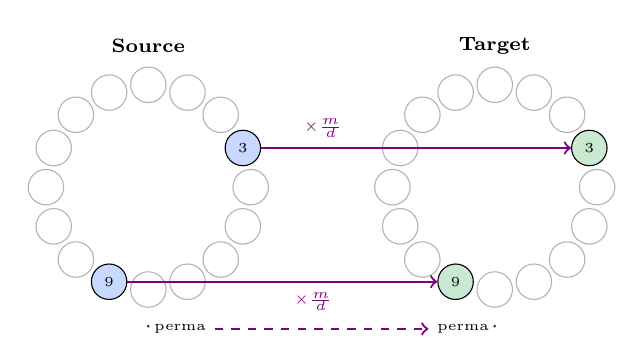
\begin{tikzpicture}[
    slot/.style={draw, minimum size=0.45cm, circle, font=\tiny, inner sep=0pt},
    active/.style={slot, fill=primaryblue!25},
    recv/.style={slot, fill=successgreen!25},
    empty/.style={slot, draw=codegray!60},
]
    % Source ring
    \begin{scope}[xshift=-2.2cm]
    \node[font=\scriptsize] at (0,1.8) {\textbf{Source}};
    \foreach \i in {0,1,2,4,5,6,7,8,10,11,12,13,14,15} {
        \pgfmathsetmacro{\angle}{90 - \i * 22.5}
        \node[empty] (s\i) at (\angle:1.3cm) {};
    }
    \foreach \i in {3,9} {
        \pgfmathsetmacro{\angle}{90 - \i * 22.5}
        \node[active] (s\i) at (\angle:1.3cm) {\i};
    }
    \end{scope}
    % Target ring
    \begin{scope}[xshift=2.2cm]
    \node[font=\scriptsize] at (0,1.8) {\textbf{Target}};
    \foreach \i in {0,1,2,4,5,6,7,8,10,11,12,13,14,15} {
        \pgfmathsetmacro{\angle}{90 - \i * 22.5}
        \node[empty] (t\i) at (\angle:1.3cm) {};
    }
    \foreach \i in {3,9} {
        \pgfmathsetmacro{\angle}{90 - \i * 22.5}
        \node[recv] (t\i) at (\angle:1.3cm) {\i};
    }
    \end{scope}
    % Transfer arrows
    \draw[->, thick, codepurple] (s3) -- node[above, font=\tiny, pos=0.2] {$\times\frac{m}{d}$} (t3);
    \draw[->, thick, codepurple] (s9) -- node[below, font=\tiny, pos=0.6] {$\times\frac{m}{d}$} (t9);
    % Perma arrow (narrowed: dots at slot-8 centers, labels inside)
    \node[font=\tiny, inner sep=0pt, anchor=west] (pleft) at ([xshift=2pt]-2.2,-1.8) {perma};
    \node[circle, fill=codepurple, inner sep=0.4pt] at ([xshift=-2pt,yshift=1pt]pleft.west|-pleft.center) {};
    \node[font=\tiny, inner sep=0pt, anchor=east] (pright) at ([xshift=-2pt]2.2,-1.8) {perma};
    \node[circle, fill=codepurple, inner sep=0.4pt] at ([xshift=2pt,yshift=1pt]pright.east|-pright.center) {};
    \draw[->, thick, dashed, codepurple] ([xshift=3pt]pleft.east) -- ([xshift=-3pt]pright.west);
\end{tikzpicture}
\caption{\texttt{push()} --- proportional transfer of locks from source to target. Each active slot is fractionally moved; permanent locks transfer separately.}
\label{fig:push}
\end{figure}

Transferring locks between two users must preserve both the amounts \emph{and} their expiry schedule.  \texttt{push()} achieves this by walking the source's bitmap and moving a proportional fraction $m/d$ of each slot's value into the corresponding slot of the target---same epoch, same remaining duration.  The fraction is rounded down per slot to keep all values integral.

\textbf{Algorithm.}
\begin{enumerate}[leftmargin=*, nosep]
\item Walk source bitmap: for each slot, compute $\Delta v = \lfloor v \cdot m / d \rfloor$.
\item Set target slot: if same epoch $\to$ accumulate, else overwrite.
\item Set source slot: subtract~$\Delta v$; clear bit if zero.
\item Batch-write both \texttt{coded} words.
\end{enumerate}

\textbf{Precondition}: Caller \textbf{must} call \texttt{free(tgt)} before \texttt{push()} to avoid stale-slot corruption (see Theorem~\ref{thm:push-corruption}).

\textbf{Complexity}: $2k$~\texttt{SLOAD}s + $2k$~\texttt{SSTORE}s + 4~\texttt{SSTORE}s (perma$\times$2, coded$\times$2).

% ---------- 4.4 stateAt() ----------
\subsection{\texttt{stateAt(user, stamp)} --- $O(k)$ Exact Query}
\label{subsec:stateat}

\begin{figure}[htbp]
\centering
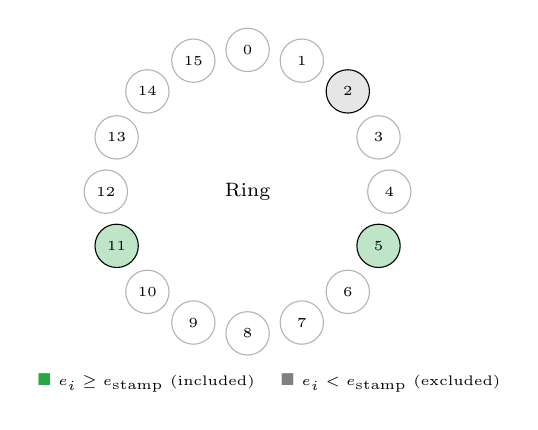
\begin{tikzpicture}[
    slot/.style={draw, minimum size=0.55cm, circle, font=\tiny, inner sep=0pt},
    included/.style={slot, fill=successgreen!30},
    excluded/.style={slot, fill=codegray!20},
    empty/.style={slot, draw=codegray!60},
]
    \foreach \i in {0,1,3,4,6,7,8,9,10,12,13,14,15} {
        \pgfmathsetmacro{\angle}{90 - \i * 22.5}
        \node[empty] (s\i) at (\angle:1.8cm) {\i};
    }
    \foreach \i in {5,11} {
        \pgfmathsetmacro{\angle}{90 - \i * 22.5}
        \node[included] (s\i) at (\angle:1.8cm) {\i};
    }
    \pgfmathsetmacro{\angle}{90 - 2 * 22.5}
    \node[excluded] (s2) at (\angle:1.8cm) {2};
    \node[font=\scriptsize] at (0,0) {Ring};
    % Legend
    \node[font=\tiny, anchor=north west] at (-2.8,-2.2) {
        \textcolor{successgreen}{$\blacksquare$}~$e_i \geq e_{\text{stamp}}$ (included) \quad
        \textcolor{codegray}{$\blacksquare$}~$e_i < e_{\text{stamp}}$ (excluded)
    };
\end{tikzpicture}
\caption{\texttt{stateAt()} --- slots with epoch $\geq e_{\text{stamp}}$ are included in the total; earlier slots are excluded.}
\label{fig:stateat}
\end{figure}

While \texttt{totalOf()} returns a cheap cached answer, \texttt{stateAt()} computes the \emph{exact} locked balance at an arbitrary timestamp by re-scanning the ring buffer.  It includes only those slots whose epoch is at or after the query point, thereby filtering out any tokens that will have expired by that time.

\textbf{Algorithm.}
\begin{enumerate}[leftmargin=*, nosep]
\item Start with $\texttt{total} = \texttt{perma}[u]$.
\item Walk bitmap: for each active slot with $e_i \geq e_{\text{stamp}}$, add $v_i$ to total.
\item Return total.
\end{enumerate}

\textbf{Complexity}: $k$~\texttt{SLOAD}s (bitmap-guided) + 1~\texttt{SLOAD} (perma). No writes.

% ---------- 4.5 totalOf() ----------
\subsection{\texttt{totalOf(user)} --- $O(1)$ Cached Query}
\label{subsec:totalof}

Decode the upper 240 bits of \texttt{coded}: a single \texttt{SLOAD}.

\begin{remark}
\label{rem:totalof-inflation}
The cached total may include expired-but-unswept slot values. Thus $\texttt{totalOf}(u) \geq \texttt{stateAt}(u, t_{\text{now}}).\texttt{total}$. Equality is restored after \texttt{free}$(u)$.
\end{remark}

\FloatBarrier

% ==============================================================================
% 5. Time-Lock Extension (TIME_LOCK)
% ==============================================================================
\section{Time-Lock Extension}
\label{sec:timelock}

The Time-Lock layer adds the \texttt{depth} mapping to the Ring-Lock structure. Each subsection describes the delta from the corresponding Ring-Lock operation.

% ---------- 5.1 Token-Seconds Integral ----------
\subsection{The Token-Seconds Integral}
\label{subsec:integral}

Token-seconds measures total commitment depth:
\begin{equation}
\label{eq:depth-def}
D(u,t) = \sum_{i \in A} v_i \bigl((e_i{+}1)Q - t\bigr) + p \cdot L
\end{equation}
where $A$ is the set of active timed slots, $p = \texttt{perma}[u]$, and $L = 16Q$.

\begin{figure}[htbp]
\centering
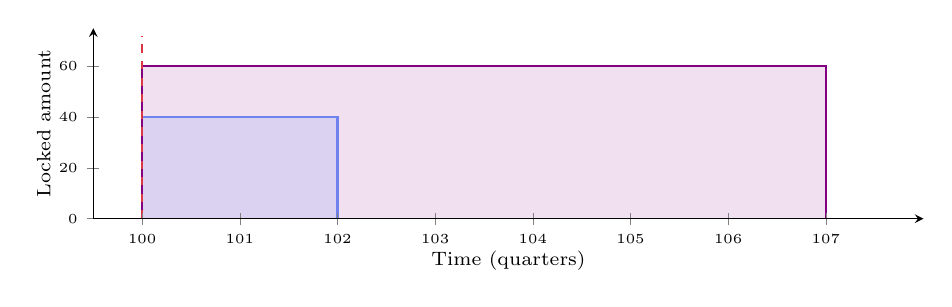
\begin{tikzpicture}
\begin{axis}[
    width=\columnwidth, height=4cm,
    xlabel={Time (quarters)},
    ylabel={Locked amount},
    xmin=99.5, xmax=108, ymin=0, ymax=75,
    xtick={100,101,102,103,104,105,106,107},
    ytick={0,20,40,60},
    axis lines=left,
    every axis x label/.style={at={(ticklabel* cs:0.5)}, anchor=north, yshift=-8pt, font=\scriptsize},
    every axis y label/.style={at={(ticklabel* cs:0.5)}, anchor=south, rotate=90, yshift=12pt, font=\scriptsize},
    tick label style={font=\tiny},
    area style,
]
    % Slot A: 40 tokens, epochs 100-102
    \addplot+[primaryblue!40, draw=primaryblue, thick, fill opacity=0.4]
        coordinates {(100,0) (100,40) (102,40) (102,0)} \closedcycle;
    % Slot B: 60 tokens, epochs 100-107
    \addplot+[codepurple!30, draw=codepurple, thick, fill opacity=0.4]
        coordinates {(100,0) (100,60) (107,60) (107,0)} \closedcycle;
    % Now line
    \draw[dashed, thick, warningred] (axis cs:100,0) -- (axis cs:100,72) node[above, font=\tiny] {$t_{\text{now}}$};
\end{axis}
\end{tikzpicture}
\caption{Token-seconds as area under the lock curve. Two timed locks: 40~tokens for 2~quarters (blue) and 60~tokens for 7~quarters (purple). Shaded area = depth.}
\label{fig:token-seconds-area}
\end{figure}

% ---------- 5.2 The O(1) Depth Identity ----------
\subsection{The $O(1)$ Depth Identity}
\label{subsec:depth-identity}

\begin{theorem}[Depth Identity]
\label{thm:depth-identity}
Let $A$ be the set of active timed slots for user~$u$, and define:
\begin{align}
\Sigma &= \textstyle\sum_{i \in A} v_i (e_i{+}1) & &\text{(stored in \texttt{depth})} \label{eq:sigma} \\
T &= \textstyle\sum_{i \in A} v_i & &\text{(timed $=$ total $-$ perma)} \label{eq:timed}
\end{align}
Then $D(u,t) = \Sigma \cdot Q - T \cdot t + p \cdot L$.
\end{theorem}

\begin{proof}
Expand the sum in~\eqref{eq:depth-def}:
\begin{align*}
D &= \sum_{i \in A} v_i \bigl((e_i{+}1)Q - t\bigr) + p L \\
  &= Q \sum_{i \in A} v_i(e_i{+}1) - t \sum_{i \in A} v_i + p L \\
  &= \Sigma Q - T t + p L \qedhere
\end{align*}
\end{proof}

\textbf{Overflow handling.} The product $T \cdot t$ can exceed 256 bits. The Solidity implementation splits the computation via OpenZeppelin's \texttt{Math.mulDiv}~\cite{oz-math}:
\begin{align}
\texttt{spent}  &= \lfloor T \cdot t / Q \rfloor \tag{\text{512-bit intermediate}} \\
\texttt{fract}  &= T \cdot t \bmod Q \tag{\text{sub-epoch remainder}} \\
\texttt{gross}  &= (\Sigma - \texttt{spent}) \cdot Q \label{eq:gross} \\
\texttt{result} &= \texttt{gross} - \texttt{fract} + p \cdot L \label{eq:result}
\end{align}

\begin{lemma}[Overflow-Safe Decomposition]
\label{lem:overflow}
Equations~\eqref{eq:gross}--\eqref{eq:result} (and the preceding \texttt{spent}/\texttt{fract} definitions) compute $\Sigma Q - T t + pL$ exactly.
\end{lemma}

\begin{proof}
Write $Tt = qQ + r$ where $q = \lfloor Tt/Q \rfloor$ and $r = Tt \bmod Q$. Then:
\[
\Sigma Q - Tt = \Sigma Q - qQ - r = (\Sigma - q)Q - r = \texttt{gross} - \texttt{fract} \qedhere
\]
\end{proof}

\begin{lemma}[$\Sigma$ and Gross Overflow Safety]
\label{lem:sigma-overflow}
Let $S$ denote the maximum per-user locked total, $E$ the current epoch, and $Q = \texttt{LOCK\_TERM}$. If $S \cdot (E{+}16) \cdot Q < 2^{256}$, then: (i)~the stored $\Sigma$ fits in \texttt{uint256}, and (ii)~the intermediate product $(\Sigma - \texttt{spent}) \cdot Q$ in \texttt{depthOf} fits in \texttt{uint256}.
\end{lemma}

\begin{proof}
All active epochs lie in $[E, E{+}15]$ (Theorem~\ref{thm:collision}), so $(e_i{+}1) \leq E{+}16$. The sum of slot values satisfies $T = \sum v_i \leq S$. Thus $\Sigma = \sum v_i(e_i{+}1) \leq S(E{+}16)$ and $(\Sigma - \texttt{spent}) \leq \Sigma$, giving $(\Sigma - \texttt{spent}) \cdot Q \leq S(E{+}16) \cdot Q < 2^{256}$.

\emph{Practical margin.} With $Q \approx 7.9 \times 10^6$ ($< 2^{23}$) and $E < 2^{32}$, the invariant holds for any per-user supply $S < 2^{201}$---far above any realistic ERC-20 token supply. The Position layer's \texttt{cap()} mechanism provides the enforcement point.
\end{proof}

\begin{figure}[htbp]
\centering
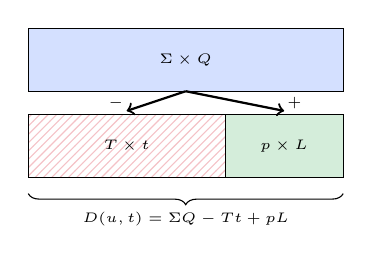
\begin{tikzpicture}[
    rect/.style={draw, minimum height=0.8cm, font=\tiny},
    label/.style={font=\tiny, anchor=north},
]
    % depth * Q
    \node[rect, fill=primaryblue!20, minimum width=4cm] (dq) at (0,0) {$\Sigma \times Q$};
    % timed * t (subtracted) — left-aligned with blue box
    \node[rect, fill=warningred!15, minimum width=2.5cm, pattern=north east lines, pattern color=warningred!30] (tt) at (-0.75,-1.1) {$T \times t$};
    % perma * LT (added) — right-aligned with blue box, abutting red box
    \node[rect, fill=successgreen!20, minimum width=1.5cm] (pl) at (1.25,-1.1) {$p \times L$};
    % Result brace — aligned with blue box edges
    \draw[decorate, decoration={brace, amplitude=4pt, mirror}] (-2,-1.7) -- (2,-1.7)
        node[midway, below, font=\tiny, yshift=-3pt] {$D(u,t) = \Sigma Q - Tt + pL$};
    % Labels
    \node[label] at (dq.south) {};
    \draw[->, thick] (0,-0.4) -- (-0.75,-0.65);
    \node[font=\tiny, anchor=east, inner sep=1pt] at (-0.75,-0.55) {$-$};
    \draw[->, thick] (0,-0.4) -- (1.25,-0.65);
    \node[font=\tiny, anchor=west, inner sep=1pt] at (1.25,-0.55) {$+$};
\end{tikzpicture}
\caption{\texttt{depthOf()} --- geometric decomposition of the $O(1)$ depth reconstruction. The large rectangle $\Sigma Q$ is reduced by $Tt$ and augmented by $pL$.}
\label{fig:depthof-geometry}
\end{figure}

% ---------- 5.3 more() with Depth ----------
\subsection{\texttt{more()} with Depth Tracking}
\label{subsec:more-depth}

When a new lock is added, the cached depth accumulator $\Sigma$ must reflect the change.  If the target slot was stale, its old contribution is first subtracted; then the new tokens' contribution---weighted by their expiry epoch---is added.  This mirrors the self-healing logic of the base \texttt{more()}, extended to one additional storage word.

\textbf{Delta from \S\ref{subsec:more}}: Step~0 (permanent sentinel) returns before reaching the depth update---\texttt{depth} is untouched for permanent locks. For timed locks, after the slot write, update \texttt{ls.depth[user]}:
\begin{itemize}[nosep]
\item Stale overwrite: $\Sigma \mathrel{-}= v_{\text{old}} \cdot (e_{\text{old}}{+}1)$.
\item Then: $\Sigma \mathrel{+}= \texttt{amount} \cdot (e_{\text{new}}{+}1)$.
\end{itemize}

\textbf{Complexity}: 3~\texttt{SSTORE}s (slot + coded + depth). Permanent: 2~\texttt{SSTORE}s (same as Ring-Lock---depth unchanged for permanent locks).

% ---------- 5.4 free() with Depth ----------
\subsection{\texttt{free()} with Depth Tracking}
\label{subsec:free-depth}

As expired slots are swept away, their epoch-weighted contributions must also leave the depth accumulator.  The sweep piggybacks on the same bitmap walk: each deleted slot's $v_i(e_i{+}1)$ term is collected into a single delta, then subtracted in one storage write at the end.

\textbf{Delta from \S\ref{subsec:free}}: Accumulate $\Delta\Sigma = \sum_{\text{expired}} v_i(e_i{+}1)$ during the sweep. After the loop: $\texttt{depth}[u] \mathrel{-}= \Delta\Sigma$.

\textbf{Complexity}: $k$~\texttt{SSTORE}s (slots) + 2~\texttt{SSTORE}s (coded + depth).

% ---------- 5.5 push() with Depth ----------
\subsection{\texttt{push()} with Depth Tracking}
\label{subsec:push-depth}

Because depth is an additive quantity, transferring locks between users is a zero-sum operation on $\Sigma$: whatever epoch-weighted value leaves the source's accumulator enters the target's.  The loop collects the total delta once, then applies symmetric updates to both depth words.

\textbf{Delta from \S\ref{subsec:push}}: Within the source-bitmap loop, accumulate $\Delta\Sigma = \sum \Delta v_i \cdot (e_i{+}1)$. After the loop:
\begin{align*}
\texttt{depth}[\texttt{src}] &\mathrel{-}= \Delta\Sigma \\
\texttt{depth}[\texttt{tgt}] &\mathrel{+}= \Delta\Sigma
\end{align*}

\textbf{Complexity}: $2k$~\texttt{SSTORE}s + 6~\texttt{SSTORE}s (perma$\times$2, coded$\times$2, depth$\times$2).

% ---------- 5.6 stateAt() with Depth ----------
\subsection{\texttt{stateAt()} with Depth}
\label{subsec:stateat-depth}

The exact query now returns a depth alongside the total.  For each included slot the remaining token$\cdot$seconds contribution $(e_i{+}1)Q - t_{\text{eff}}$ is accumulated on the fly, plus the permanent lock's constant contribution $p \cdot L$.

\textbf{Delta from \S\ref{subsec:stateat}}: Returns $(\texttt{total}, \texttt{depth})$. For each active slot with $e_i \geq e_{\text{stamp}}$:
\[
\texttt{depth} \mathrel{+}= v_i \bigl((e_i{+}1)Q - t_{\text{eff}}\bigr)
\]
where $t_{\text{eff}} = \max(t_{\text{stamp}}, t_{\text{now}})$. Permanent contribution: $\texttt{depth} \mathrel{+}= p \cdot L$.

\textbf{Complexity}: $k$~\texttt{SLOAD}s + multiply/add per slot. No additional storage reads.

% ---------- 5.7 depthOf() ----------
\subsection{\texttt{depthOf(user)} --- $O(1)$ Cached Depth}
\label{subsec:depthof}

This is the key operation.  Rather than looping over every active slot, \texttt{depthOf()} reconstructs the exact token-seconds value from three cached storage words ($\Sigma$, $T$, $p$) and the current timestamp, using the Depth Identity $D = \Sigma Q - Tt + pL$.  The only subtlety is avoiding 256-bit overflow in the product $Tt$: the function splits it into a quotient via \texttt{mulDiv} and a remainder via \texttt{mulmod}, keeping all intermediate values within range.  The result is a single $O(1)$ read with no loops and no bitmap traversal.

Full algorithm:

\begin{lstlisting}[language=Solidity, caption={\texttt{depthOf} implementation}, label={lst:depthof}]
function depthOf(Lock storage ls, address user)
    internal view returns (uint256)
{
    (uint240 total,) = _de(ls.coded[user]);
    uint256 perma = ls.perma[user];
    uint256 depth = ls.depth[user];
    uint256 timed = sub256(total, perma);
    uint256 spent = Math.mulDiv(
        timed, block.timestamp, LOCK_TERM);
    uint256 fract = mulmod(
        timed, block.timestamp, LOCK_TERM);
    uint256 gross = mul256(
        sub256(depth, spent), LOCK_TERM);
    return add256(
        sub256(gross, fract),
        mul256(perma, LOCK_TIME));
}
\end{lstlisting}

\textbf{Complexity}: 3~\texttt{SLOAD}s (\texttt{coded}, \texttt{perma}, \texttt{depth}). No loops, no bitmap iteration.

\FloatBarrier

% ---------- Worked Example ----------
\subsection{Worked Example}
\label{subsec:worked-example}

\begin{definition}[Setup]
$Q = 7{,}889{,}400$\,s, $t = 100Q$ (start of epoch~100). Lock 40~tokens for 1\,Q (epoch~101, slot~$101 \bmod 16 = 5$) and 60~tokens for 6\,Q (epoch~106, slot~$106 \bmod 16 = 10$). No permanent locks.
\end{definition}

Stored values:
\begin{align*}
\Sigma &= 40 \times 102 + 60 \times 107 = 4{,}080 + 6{,}420 = 10{,}500 \\
T &= 100 \quad (\text{timed} = 100, \; p = 0) \\
t &= 100Q
\end{align*}

\textbf{Via \texttt{depthOf}} ($O(1)$):
\begin{align*}
D &= \Sigma Q - Tt + pL \\
  &= 10{,}500Q - 100 \cdot 100Q + 0 \\
  &= 10{,}500Q - 10{,}000Q = 500Q \text{ token-seconds}
\end{align*}

\textbf{Via \texttt{stateAt}} ($O(k)$, verification):
\begin{align*}
\text{slot 5:}\quad & 40 \times (102Q - 100Q) = 80Q \\
\text{slot 10:}\quad & 60 \times (107Q - 100Q) = 420Q \\
\text{total:}\quad & 80Q + 420Q = 500Q \;\checkmark
\end{align*}

% ==============================================================================
% 6. Invariants and Correctness Proofs
% ==============================================================================
\section{Invariants and Correctness Proofs}
\label{sec:proofs}

% ---------- 6.1 Collision Freedom ----------
\subsection{Collision Freedom}

\begin{theorem}[Collision Freedom]
\label{thm:collision}
For any user~$u$ and any two active (non-expired) locks in slots~$i$ and~$j$ with epochs~$e_i$ and~$e_j$: if $e_i \bmod 16 = e_j \bmod 16$, then $e_i = e_j$.
\end{theorem}

\begin{proof}
By the \texttt{more()} require guard (step~1), $\texttt{dt\_term} \leq L - Q = 15Q$. A lock created at time~$t$ targets epoch $e = \lfloor(t{+}\texttt{dt\_term})/Q\rfloor$. The current epoch is $e_{\text{now}} = \lfloor t/Q \rfloor$. Thus:
\[
e_{\text{now}} \leq e \leq \left\lfloor \frac{t + 15Q}{Q} \right\rfloor = \left\lfloor \frac{t}{Q} \right\rfloor + 15 = e_{\text{now}} + 15
\]
All active epochs lie in a window of at most 16 consecutive integers $[e_{\text{now}}, e_{\text{now}}{+}15]$. Two distinct integers in this window with the same residue mod~16 must differ by at least~16. However, the maximum difference between any two elements of $[e_{\text{now}}, e_{\text{now}}{+}15]$ is $15 < 16$---a contradiction.
\end{proof}

\begin{corollary}[Cross-User Collision]
\label{cor:cross-user}
When \texttt{push(src, tgt)} copies a lock from source slot~$i$ to target slot~$i$, and the target already has an active lock at index~$i$, then the target epoch must equal the source epoch (since both are active and share the same mod-16 index). The \texttt{\_setTarget} accumulate-path is therefore always taken for active target slots; empty or swept target slots take the overwrite path.
\end{corollary}

\begin{proof}
Follows directly from Theorem~\ref{thm:collision} applied to the target user's active set augmented with the incoming epoch.
\end{proof}

% ---------- 6.2 Depth Identity Correctness ----------
\subsection{Depth Identity Correctness}

\begin{theorem}[Depth Identity]
\label{thm:depth-correct}
After \texttt{free(u)}, $\texttt{depthOf}(u) = \texttt{stateAt}(u, t_{\text{now}}).\texttt{depth}$.
\end{theorem}

\begin{proof}
By Theorem~\ref{thm:depth-identity}, $D = \Sigma Q - Tt + pL$. After \texttt{free()}, the expired set $E = \emptyset$, so the stored $\Sigma$ and $T$ exactly represent the active set~$A$. The identity reconstructs $D$ identically to the sum in~\eqref{eq:depth-def}.
\end{proof}

% ---------- 6.3 Cached vs Exact ----------
\subsection{Cached vs Exact Invariants}

\begin{theorem}[Total Inflation]
\label{thm:total-inflation}
$\texttt{totalOf}(u) \geq \texttt{stateAt}(u, t_{\text{now}}).\texttt{total}$ at all times.
\end{theorem}

\begin{proof}
\texttt{totalOf} returns the \texttt{total} from \texttt{coded}, which includes contributions from all slots with set bitmap bits---both active and expired. \texttt{stateAt} sums only slots with $e_i \geq e_{\text{now}}$. Since every active slot is counted by both, and expired slots are counted only by \texttt{totalOf}:
\begin{align*}
\texttt{totalOf}(u) &= \texttt{stateAt}(u,t_{\text{now}}).\texttt{total} + \textstyle\sum_{i \in E} v_i \\
                     &\geq \texttt{stateAt}(u,t_{\text{now}}).\texttt{total} \qedhere
\end{align*}
\end{proof}

\begin{theorem}[Depth Deflation]
\label{thm:depth-deflation}
$\texttt{depthOf}(u) \leq \texttt{stateAt}(u, t_{\text{now}}).\texttt{depth}$ at all times.
\end{theorem}

\begin{proof}
Let $E$ be the set of expired slots still in the bitmap, $A$ the active set. Decompose:
\begin{align*}
\texttt{depthOf}(u) &= \Sigma Q - Tt + pL \\
    &= \underbrace{[\Sigma_A Q - T_A t + pL]}_{\texttt{stateAt}.depth} + \underbrace{[\Sigma_E Q - T_E t]}_{\leq\, 0}
\end{align*}
For each expired slot $i \in E$: $e_i < e_{\text{now}} = \lfloor t/Q \rfloor$, so $(e_i{+}1)Q \leq t$, giving $v_i((e_i{+}1)Q - t) \leq 0$.
\end{proof}

\begin{theorem}[Equality After Free]
\label{thm:equality-after-free}
After \texttt{free(u)}: $\texttt{totalOf}(u) = \texttt{stateAt}(u, t_{\text{now}}).\texttt{total}$ and $\texttt{depthOf}(u) = \texttt{stateAt}(u, t_{\text{now}}).\texttt{depth}$.
\end{theorem}

\begin{proof}
\texttt{free()} deletes every slot with $e_i < e_{\text{now}}$, making $E = \emptyset$. The expired-set contributions in Theorems~\ref{thm:total-inflation} and~\ref{thm:depth-deflation} vanish.
\end{proof}

\begin{figure}[htbp]
\centering
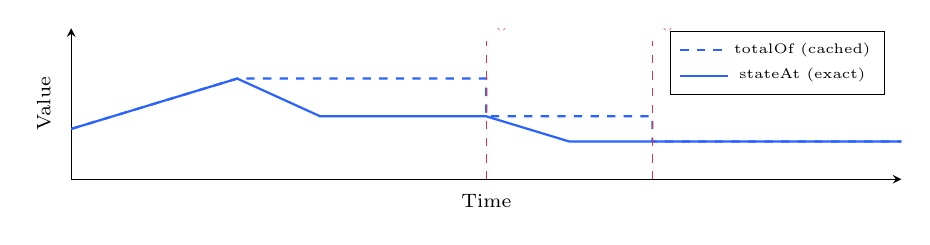
\begin{tikzpicture}
\begin{axis}[
    width=\columnwidth, height=3.5cm,
    xlabel={Time},
    ylabel={Value},
    xmin=0, xmax=10, ymin=0, ymax=1.2,
    xtick=\empty, ytick=\empty,
    axis lines=left,
    every axis x label/.style={at={(ticklabel* cs:0.5)}, anchor=north, yshift=-2pt, font=\scriptsize},
    every axis y label/.style={at={(ticklabel* cs:0.5)}, anchor=south, rotate=90, yshift=4pt, font=\scriptsize},
    legend style={font=\tiny, at={(0.98,0.98)}, anchor=north east},
]
    % totalOf (cached, stays high)
    \addplot[primaryblue, thick, dashed] coordinates {(0,0.4) (2,0.8) (3,0.8) (4,0.8) (5,0.8) (5,0.5) (6,0.5) (7,0.5) (7,0.3) (10,0.3)};
    \addlegendentry{totalOf (cached)}
    % stateAt.total (drops at expiry)
    \addplot[primaryblue, thick] coordinates {(0,0.4) (2,0.8) (3,0.5) (5,0.5) (5,0.5) (6,0.3) (7,0.3) (10,0.3)};
    \addlegendentry{stateAt (exact)}
    % free() events
    \draw[dashed, warningred, thin] (axis cs:5,0) -- (axis cs:5,1.1) node[above, font=\tiny] {free()};
    \draw[dashed, warningred, thin] (axis cs:7,0) -- (axis cs:7,1.1) node[above, font=\tiny] {free()};
\end{axis}
\end{tikzpicture}
\caption{Cached \texttt{totalOf} remains inflated above the exact \texttt{stateAt} value until \texttt{free()} sweeps expired slots, restoring equality.}
\label{fig:cached-vs-exact}
\end{figure}

% ---------- 6.4 Self-Healing ----------
\subsection{Self-Healing Correctness}

\begin{theorem}[Self-Healing]
\label{thm:self-healing}
If \texttt{more(u, amount, dt\_term)} overwrites a stale slot at index~$i$, then after the operation, the cached \texttt{total} and \texttt{depth} are consistent with the new slot value.
\end{theorem}

\begin{proof}
When \texttt{more()} finds $e_{\text{slot}} \neq e_{\text{target}}$ and $v_{\text{slot}} > 0$:
\begin{enumerate}[nosep]
\item $\Sigma \mathrel{-}= v_{\text{old}}(e_{\text{old}}{+}1)$; $T \mathrel{-}= v_{\text{old}}$.
\item Overwrite slot: $e \leftarrow e_{\text{target}}$, $v \leftarrow \texttt{amount}$.
\item $\Sigma \mathrel{+}= \texttt{amount} \cdot (e_{\text{target}}{+}1)$; $T \mathrel{+}= \texttt{amount}$.
\end{enumerate}
The net effect is as if the stale slot had been freed first, then the new lock created.
\end{proof}

\begin{remark}
Self-healing is per-slot. Other stale slots remain uncorrected until \texttt{free()} or their own overwrite by a future \texttt{more()}.
\end{remark}

% ---------- 6.5 Push Depth Conservation ----------
\subsection{Depth Conservation Under Push}

\begin{theorem}[Push Depth Conservation]
\label{thm:push-conservation}
Let $D_{\text{before}} = \texttt{depthOf}(\texttt{src}) + \texttt{depthOf}(\texttt{tgt})$ before the call. After \texttt{push(src, tgt, m, d)} with prior \texttt{free(src)} and \texttt{free(tgt)}:
\[
\texttt{depthOf}(\texttt{src}) + \texttt{depthOf}(\texttt{tgt}) = D_{\text{before}}
\]
That is, the combined depth is exactly conserved.
\end{theorem}

\begin{proof}
For each source slot, $\Delta v = \lfloor v \cdot m/d \rfloor$ is subtracted from \texttt{depth[src]} and added to \texttt{depth[tgt]} as $\Delta v \cdot (e{+}1)$. The same $\Delta v$ is subtracted from $T_{\text{src}}$ and added to $T_{\text{tgt}}$. Thus the aggregate $\Sigma = \Sigma_{\text{src}} + \Sigma_{\text{tgt}}$ and $T = T_{\text{src}} + T_{\text{tgt}}$ are each invariant across the transfer. Since both users were freed, $D_{\text{src}} + D_{\text{tgt}} = (\Sigma_{\text{src}} + \Sigma_{\text{tgt}})Q - (T_{\text{src}} + T_{\text{tgt}})t + (p_{\text{src}} + p_{\text{tgt}})L$, and all three aggregate terms are unchanged.
\end{proof}

\begin{remark}
While the combined depth is exactly conserved, the \emph{split} between source and target is subject to integer rounding: each slot transfers $\lfloor v \cdot m/d \rfloor$ instead of the ideal $v \cdot m/d$. The per-slot depth rounding error is $\epsilon_i \cdot ((e_i{+}1)Q - t)$ where $\epsilon_i < 1$, bounded by $16Q$ per slot since $(e_i{+}1)Q - t < 16Q$ for all active slots. The aggregate rounding error across $k$ active slots is therefore bounded by $k \cdot 16Q \leq 256Q$. For typical operations with $k = 1$--$3$ active slots, this is negligible relative to lock values of order~$10^{18}$.
\end{remark}

% ---------- 6.6 Stale-Slot Corruption ----------
\subsection{Stale-Slot Corruption Without Free}

\begin{theorem}[Push Corruption]
\label{thm:push-corruption}
If \texttt{push(src, tgt, m, d)} is called without prior \texttt{free(tgt)}, and the target has a stale slot at index~$i$ that is overwritten by an incoming active slot, then:
\begin{enumerate}[nosep]
\item \texttt{totalOf(tgt)} is permanently inflated by the stale slot's value.
\item \texttt{depthOf(tgt)} is permanently corrupted.
\item Subsequent \texttt{free(tgt)} cannot recover correctness, because the stale epoch was overwritten with an active epoch.
\end{enumerate}
\end{theorem}

\begin{proof}
The stale target slot has $(e_{\text{stale}}, v_{\text{stale}})$ with $e_{\text{stale}} < e_{\text{now}}$. When \texttt{\_setTarget} finds $e_{\text{slot}} \neq e_{\text{incoming}}$, it overwrites: $v \leftarrow \Delta v$, $e \leftarrow e_{\text{incoming}}$. The overwritten $v_{\text{stale}}$ was still counted in \texttt{coded[tgt]} and \texttt{depth[tgt]}, but is now lost---\texttt{free()} will see the new active epoch and skip the slot.
\end{proof}

\begin{remark}
This is a known design constraint. The \texttt{push()} function requires the \texttt{free(tgt)} precondition. The Position layer enforces it via \texttt{\_lockFree(from, to)} before \texttt{\_lockPush()}.
\end{remark}

% ---------- 6.7 Non-Negativity ----------
\subsection{Non-Negativity}

\begin{theorem}[Depth Non-Negativity]
\label{thm:non-negativity}
$\texttt{stateAt}(u, t).\texttt{depth} \geq 0$ for all users and timestamps $t \geq t_{\text{now}}$. $\texttt{depthOf}(u) \geq 0$ when saturating arithmetic is used.
\end{theorem}

\begin{proof}
\textbf{For \texttt{stateAt}} ($t \geq t_{\text{now}}$): The effective time is $t_{\text{eff}} = \max(t, t_{\text{now}}) = t$. Each included slot satisfies $e_i \geq e_{\text{stamp}} = \lfloor t/Q \rfloor$, so $(e_i{+}1)Q \geq (\lfloor t/Q \rfloor {+} 1)Q > t$. Each term $v_i((e_i{+}1)Q - t) > 0$. The permanent contribution $pL \geq 0$.

\textbf{For \texttt{depthOf}}: When expired slots exist, the expired contribution is negative (Theorem~\ref{thm:depth-deflation}), potentially driving the total negative. Saturating arithmetic (\texttt{sub256}) clamps to zero.
\end{proof}

% ---------- 6.8 Bitmap Consistency ----------
\subsection{Bitmap Consistency}

\begin{theorem}[Bitmap Invariant]
\label{thm:bitmap}
A bitmap bit at index~$i$ is set if and only if $\texttt{slots}[u][i].\texttt{value} > 0$.
\end{theorem}

\begin{proof}
By induction on operations:
\begin{itemize}[nosep]
\item \textbf{Base}: All slots zero-initialized, bitmap $= 0$.
\item \textbf{\texttt{more()}}: Sets bit~$i$ when writing a non-zero value.
\item \textbf{\texttt{free()}}: Clears bit~$i$ only when deleting slot~$i$ (value $\to 0$).
\item \textbf{\texttt{push()} source}: \texttt{\_setSource} returns $\lnot\texttt{mask}(i)$ (clearing bit) only when $v = 0$ after subtraction.
\item \textbf{\texttt{push()} target}: \texttt{\_setTarget} returns $\texttt{mask}(i)$ (setting bit), and the loop skips $\Delta v = 0$.
\end{itemize}
In all cases the invariant is preserved.
\end{proof}

% ---------- 6.9 Permanent Lock Invariance ----------
\subsection{Permanent Lock Invariance}

\begin{theorem}[Permanent Depth Independence]
\label{thm:perma-independence}
The \texttt{depth} register is independent of permanent locks. Permanent contributions to token-seconds are computed at query time as $p \cdot L$.
\end{theorem}

\begin{proof}
In \texttt{more()} with $\texttt{dt\_term} = 2^{256}{-}1$: only \texttt{perma} and \texttt{coded} are updated; \texttt{depth} is untouched. In \texttt{free()}: only timed slots are swept. In \texttt{push()}: \texttt{\_movPerma} transfers between \texttt{perma[src]} and \texttt{perma[tgt]} without touching \texttt{depth}. The \texttt{depth} register exclusively tracks $\sum v_i(e_i{+}1)$ for timed slots.
\end{proof}

\FloatBarrier

% ==============================================================================
% 7. Gas Analysis
% ==============================================================================
\section{Gas Analysis}
\label{sec:gas}

Table~\ref{tab:gas} summarizes the storage access costs for each operation under both the Ring-Lock base layer and the Time-Lock extension.

\begin{table}[htbp]
\centering
\caption{Storage access costs per operation.}
\label{tab:gas}
\small
\begin{tabular*}{0.95\columnwidth}{@{\extracolsep{\fill}}lccc@{}}
\toprule
Operation & Ring-Lock & Time-Lock & $\Delta$ \\
\midrule
\texttt{more} (timed) & 2 \texttt{SSTORE} & 3 \texttt{SSTORE} & $+1$ \\
\texttt{more} (perma) & 2 \texttt{SSTORE} & 2 \texttt{SSTORE} & $0$ \\
\texttt{free} & $k{+}1$ \texttt{SSTORE} & $k{+}2$ \texttt{SSTORE} & $+1$ \\
\texttt{push} & $2k{+}4$ \texttt{SSTORE} & $2k{+}6$ \texttt{SSTORE} & $+2$ \\
\texttt{totalOf} & 1 \texttt{SLOAD} & 1 \texttt{SLOAD} & $0$ \\
\texttt{depthOf} & --- & 3 \texttt{SLOAD} & new \\
\texttt{stateAt} & $k{+}1$ \texttt{SLOAD} & $k{+}1$ \texttt{SLOAD} & $0$ \\
\bottomrule
\end{tabular*}
\end{table}

The Time-Lock extension adds at most 2~\texttt{SSTORE}s per mutating operation. All queries remain bounded. The $O(1)$ \texttt{depthOf} avoids the $O(k)$ \texttt{stateAt} walk for the common case of checking a user's commitment depth---the primary use case for interest rate adjustments.

Since $k \leq 16$ (ring-buffer width), even the worst-case \texttt{push()} has a hard upper bound of 38~\texttt{SSTORE}s and 38~\texttt{SLOAD}s ($2k$ slots $+$ 6 ancillary: \texttt{coded}$\times$2, \texttt{perma}$\times$2, \texttt{depth}$\times$2), ensuring gas predictability regardless of user behavior.

% ==============================================================================
% 8. Integration
% ==============================================================================
\section{Integration}
\label{sec:integration}

\subsection{Position Layer}

The \texttt{Position} contract wraps the \texttt{Lock} library, maintaining a parallel lock as a global total tracker:

\begin{itemize}[nosep]
\item \texttt{\_lockMore(user, amount, dt\_term)}: calls \texttt{lock.more()} for \texttt{user} \emph{and} the global total.
\item \texttt{\_lockFree(from, to)}: sweeps expired slots for source, target, \emph{and} the global total before any transfer---enforcing the \texttt{free(tgt)} precondition of Theorem~\ref{thm:push-corruption}.
\item \texttt{\_lockPush(from, to, amount)}: proportional lock transfer during position transfer, with fraction $m/d = \texttt{amount}/\texttt{balance}$.
\end{itemize}

\subsection{Graduated Lock Bonus/Malus}

The protocol uses the token-second depth to scale interest rates~\cite{wp}:

\begin{definition}[Lock Ratio]
\label{def:lock-ratio}
\[
\lambda(u) = \frac{\texttt{depthOf}(u)}{\texttt{balanceOf}(u) \cdot L}
\]
where $\lambda \in [0,1]$ measures normalized commitment depth.
\end{definition}

Interest rate adjustments:
\begin{align}
\text{Supply:} \quad r_{\text{eff}} &= r_{\text{base}} \cdot (1 + \beta_s \cdot \lambda) \label{eq:supply-bonus} \\
\text{Borrow:} \quad r_{\text{eff}} &= r_{\text{base}} \cdot (1 - \beta_b \cdot \lambda) \label{eq:borrow-malus}
\end{align}
where $\beta_s = \texttt{LOCK\_BONUS}$ and $\beta_b = \texttt{LOCK\_MALUS}$ are governance parameters bounded by the spread.

\begin{figure}[htbp]
\centering
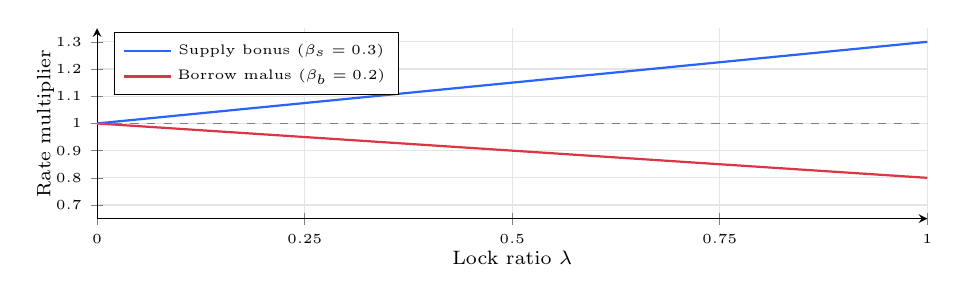
\begin{tikzpicture}
\begin{axis}[
    width=\columnwidth, height=4cm,
    xlabel={Lock ratio $\lambda$},
    ylabel={Rate multiplier},
    xmin=0, xmax=1, ymin=0.65, ymax=1.35,
    xtick={0,0.25,0.5,0.75,1.0},
    ytick={0.7,0.8,0.9,1.0,1.1,1.2,1.3},
    axis lines=left,
    every axis x label/.style={at={(ticklabel* cs:0.5)}, anchor=north, yshift=-8pt, font=\scriptsize},
    every axis y label/.style={at={(ticklabel* cs:0.5)}, anchor=south, rotate=90, yshift=12pt, font=\scriptsize},
    tick label style={font=\tiny},
    legend style={font=\tiny, at={(0.02,0.98)}, anchor=north west},
    grid=major,
    grid style={gray!20},
]
    % Supply bonus
    \addplot[primaryblue, thick, domain=0:1, samples=50] {1 + 0.3*x};
    \addlegendentry{Supply bonus ($\beta_s = 0.3$)}
    % Borrow malus
    \addplot[warningred, thick, domain=0:1, samples=50] {1 - 0.2*x};
    \addlegendentry{Borrow malus ($\beta_b = 0.2$)}
    % Base rate
    \draw[dashed, codegray] (axis cs:0,1) -- (axis cs:1,1);
\end{axis}
\end{tikzpicture}
\caption{Lock bonus/malus scaling. Suppliers with higher lock ratios earn more interest; borrowers with higher lock ratios pay less (malus subtracted from their accrued debt).}
\label{fig:lock-bonus}
\end{figure}

Supply positions benefit: locked suppliers earn bonus interest proportional to their commitment depth. Borrow positions also benefit: locked borrowers receive a malus that \emph{reduces} their effective borrowing cost, incentivizing long-term commitment on both sides of the market.

% ==============================================================================
% 9. Conclusion
% ==============================================================================
\section{Conclusion}
\label{sec:conclusion}

We have presented a ring-buffer data structure for time-locked positions with five key properties:

\begin{enumerate}[leftmargin=*, nosep]
\item A 16-slot quarterly ring buffer providing bounded storage per user (19 words).
\item Bitmap-guided $O(k)$ sweep with $k \leq 16$, ensuring gas-bounded expiry.
\item An $O(1)$ cached depth metric via the algebraic identity $D = \Sigma Q - Tt + pL$, enabling constant-time token-second queries from three stored values.
\item Proportional lock transfer in $O(k)$ for position fungibility during liquidation.
\item Integration with graduated lock bonus/malus for interest rate scaling in DeFi lending.
\end{enumerate}

The mechanism is deployed in the XPower Banq protocol~\cite{wp}, where the collision-freedom guarantee (Theorem~\ref{thm:collision}) ensures ring-buffer correctness, and the depth identity (Theorem~\ref{thm:depth-identity}) enables gas-efficient interest rate adjustments. Formal proofs of all invariants are provided in Section~\ref{sec:proofs}.

% ==============================================================================
% References
% ==============================================================================
\begin{thebibliography}{99}

\bibitem{wp}
\textsc{Karun The Ritch}.
\newblock XPower Banq: A Permissionless DeFi Lending Protocol with Lethargic Governance and Beta-Distributed Position Caps.
\newblock \emph{Preprint}, 2026.
\newblock \url{https://www.xpowerbanq.com}

\bibitem{apx}
\textsc{Karun The Ritch}.
\newblock XPower Banq: Technical Appendices.
\newblock \emph{Preprint}, 2026.
\newblock \url{https://www.xpowerbanq.com}

\bibitem{curve}
Curve Finance.
\newblock Vote-Escrowed CRV (veCRV).
\newblock \emph{Curve Documentation}, 2020.
\newblock \url{https://curve.readthedocs.io/dao-vecrv.html}

\bibitem{convex}
Convex Finance.
\newblock Vote-Locked CVX (vlCVX).
\newblock \emph{Convex Documentation}, 2021.
\newblock \url{https://docs.convexfinance.com/convexfinance/general-information/understanding-cvx/vote-locking}

\bibitem{oz-timelock}
OpenZeppelin.
\newblock TimelockController.
\newblock \emph{OpenZeppelin Contracts}, 2020.
\newblock \url{https://docs.openzeppelin.com/contracts/5.x/api/governance#TimelockController}

\bibitem{erc20}
Vogelsteller, F. and Buterin, V.
\newblock EIP-20: Token Standard.
\newblock \emph{Ethereum Improvement Proposals}, 2015.
\newblock \url{https://eips.ethereum.org/EIPS/eip-20}

\bibitem{erc4626}
Joey Santoro et al.
\newblock EIP-4626: Tokenized Vault Standard.
\newblock \emph{Ethereum Improvement Proposals}, 2022.
\newblock \url{https://eips.ethereum.org/EIPS/eip-4626}

\bibitem{debruijn}
de~Bruijn, N.G.
\newblock A combinatorial problem.
\newblock \emph{Proceedings of the Section of Sciences of the Koninklijke Nederlandse Akademie van Wetenschappen}, 49(7):758--764, 1946.

\bibitem{oz-math}
OpenZeppelin.
\newblock Math Library (mulDiv).
\newblock \emph{OpenZeppelin Contracts}, 2023.
\newblock \url{https://docs.openzeppelin.com/contracts/5.x/api/utils#Math}

\bibitem{ring-buffer}
Lee, P.P.C., Bu, T., and Chandranmenon, G.P.
\newblock A lock-free, cache-efficient shared ring buffer for multi-core architectures.
\newblock In \emph{Proc.\ 5th ACM/IEEE Symposium on Architectures for Networking and Communications Systems (ANCS)}, pp.\ 78--79, 2009.
\newblock \url{https://doi.org/10.1145/1882486.1882508}

\end{thebibliography}

% ==============================================================================
% Glossary
% ==============================================================================
\section*{Glossary}

\begin{description}[style=nextline, font=\normalfont\bfseries, leftmargin=1.5em]

\item[Bitmap] 16-bit mask tracking which slots contain active locks. Stored in the lower 16 bits of \texttt{coded}.

\item[Depth ($\Sigma$)] Cached epoch-weighted sum $\sum v_i(e_i{+}1)$ enabling $O(1)$ token-second reconstruction.

\item[Depth Identity] The algebraic identity $D = \Sigma Q - Tt + pL$ (Theorem~\ref{thm:depth-identity}) that converts the $O(k)$ token-seconds sum into an $O(1)$ cached computation.

\item[Epoch] Absolute quarter index $e = \lfloor t/Q \rfloor$. Each epoch spans exactly $Q$ seconds.

\item[Lock Ratio ($\lambda$)] $\texttt{depthOf}(u) / (\texttt{balanceOf}(u) \cdot L) \in [0,1]$, depth of user commitment normalized by balance and maximum lock duration.

\item[LOCK\_TERM ($Q$)] One quarter $\approx 91.3$ days---the epoch duration and ring-buffer granularity.

\item[LOCK\_TIME ($L$)] $16 \times Q \approx 48$ months---maximum lock duration and permanent lock depth cap.

\item[Lock Bonus/Malus] Interest rate scaling driven by lock depth. Suppliers earn a bonus $r_{\text{base}}(1 + \beta_s \lambda)$; borrowers receive a malus $r_{\text{base}}(1 - \beta_b \lambda)$ that reduces their effective cost (Equations~\ref{eq:supply-bonus}--\ref{eq:borrow-malus}).

\item[Permanent Lock] Irrevocable lock with $\texttt{dt\_term} = 2^{256}{-}1$. Stored in \texttt{perma}, not in a ring slot. Contributes $p \cdot L$ to token-seconds at query time.

\item[Ring-Lock] Base mechanism: ring buffer + bitmap + cached total. 18 words per user.

\item[Self-Healing] \texttt{more()} correcting stale slot contributions during overwrite, maintaining \texttt{total} and \texttt{depth} consistency per-slot (Theorem~\ref{thm:self-healing}).

\item[Time-Lock] Extension of Ring-Lock adding the \texttt{depth} mapping for token-seconds. 19 words per user.

\item[Token-Seconds] $\sum v_i \times \text{remaining time}$---integral of locked amount over remaining time. The depth metric that drives graduated commitment.

\end{description}

% Ensure even page count for duplex printing
\clearpage
\ifodd\value{page}\else\thispagestyle{empty}\null\clearpage\fi

\end{document}
